\documentclass[12pt,a4paper]{article}
\pagestyle{plain}
\usepackage{fullpage}
\usepackage[english]{babel}
\usepackage{enumerate}

%equations
\usepackage[fleqn]{amsmath}
\numberwithin{equation}{section}

%figures
\usepackage[dvips]{graphicx}
\graphicspath{{./images/}}
\numberwithin{figure}{section}

%excercises
\newcounter{Exercise}
\setcounter{Exercise}{1}
\usepackage[dvipsnames]{xcolor}
\usepackage{framed}
\definecolor{shadecolor}{gray}{0.9}
\usepackage{caption}

%tables
\numberwithin{table}{section}

%specials
\usepackage{textcomp} %special (greek) characters as text
%\usepackage{pstricks} %
%\usepackage{ifthen} %
%\usepackage{calc} %
%\usepackage{isotope}
\usepackage{hyperref}
\usepackage[bottom]{footmisc} %footnote below figure
\usepackage{footnpag}%number footnotes per page


%document details
\author{Koos Kortland \\ translated and adapted by K. Schadenberg}
\date{}
\title{Primary Particle - Angle}


\begin{document}
\maketitle

\section{Introduction}
From the measured arrival times of the air shower at at least three HiSPARC detector stations one can calculate the direction of travel of the air shower. From this the direction of travel of the primary cosmic ray can be deduced. The data from the detectors consist of a position and a time coordinate. In this module will look at how we can used this data to calculate the primary particle direction.

\section{The Data}
In this text we will use the following notation:
\begin{enumerate}[-]
\item Indices (in subscript) will denote the station, stations are assigned a letter (A, B, etc.).
\item The location of station A is given by the position coordinates: $x_A$ and $y_A$.\footnote{At the moment we will not look at the height of the detectors, e.g. $z_A$. At a later stage you might want to included this parameter to improve the accurace of the calculation.}
\item The letter $t$ denotes the arrival time of the shower, $t_B$ is the arrival time of the shower at detector B.
\end{enumerate}
If we have three detectors, A, B, and C, we have the following data set: $A(x_A, y_A, t_A)$, $B(x_B, y_B, t_B)$, and $C(x_C, y_C, t_C)$. In this text we will answer the question: How can we determine the direction of the primary particle from this data?

\section{Framing the problem}
The direction of the primary cosmic ray can be described using two angles: the zenith and azimuth angle. In the following calculations we assume that the trajectory of the ray is straight (i.e. not curved) and that the air shower follows the same path as the primary particle. It is as though we draw a line from the first collision of the primary particle all the way down to the surface of the Earth, which is in line with the path of the primary particle. We call this line b, see figure~\ref{fig:shower_angles}.

The angle between the line b and the vertical Z-axis is the zenith angle $\theta$. The azimuth angle $\varphi$ is the angle between the projection of b onto the XY-plane (the Earth surface) and the horizontal X-axis. The projection of the line b is called b'. Care must be taken when naming the directions. We choose to call the positive X-direction West and the negative X-direction East. This means that the positive Y-direction is South. With the two angles $\theta$ and $\varphi$ we can completely describe the direction of travel of the cosmic ray. Both angles are also drawn in figure~\ref{fig:shower_angles}.

\begin{figure}\begin{center}
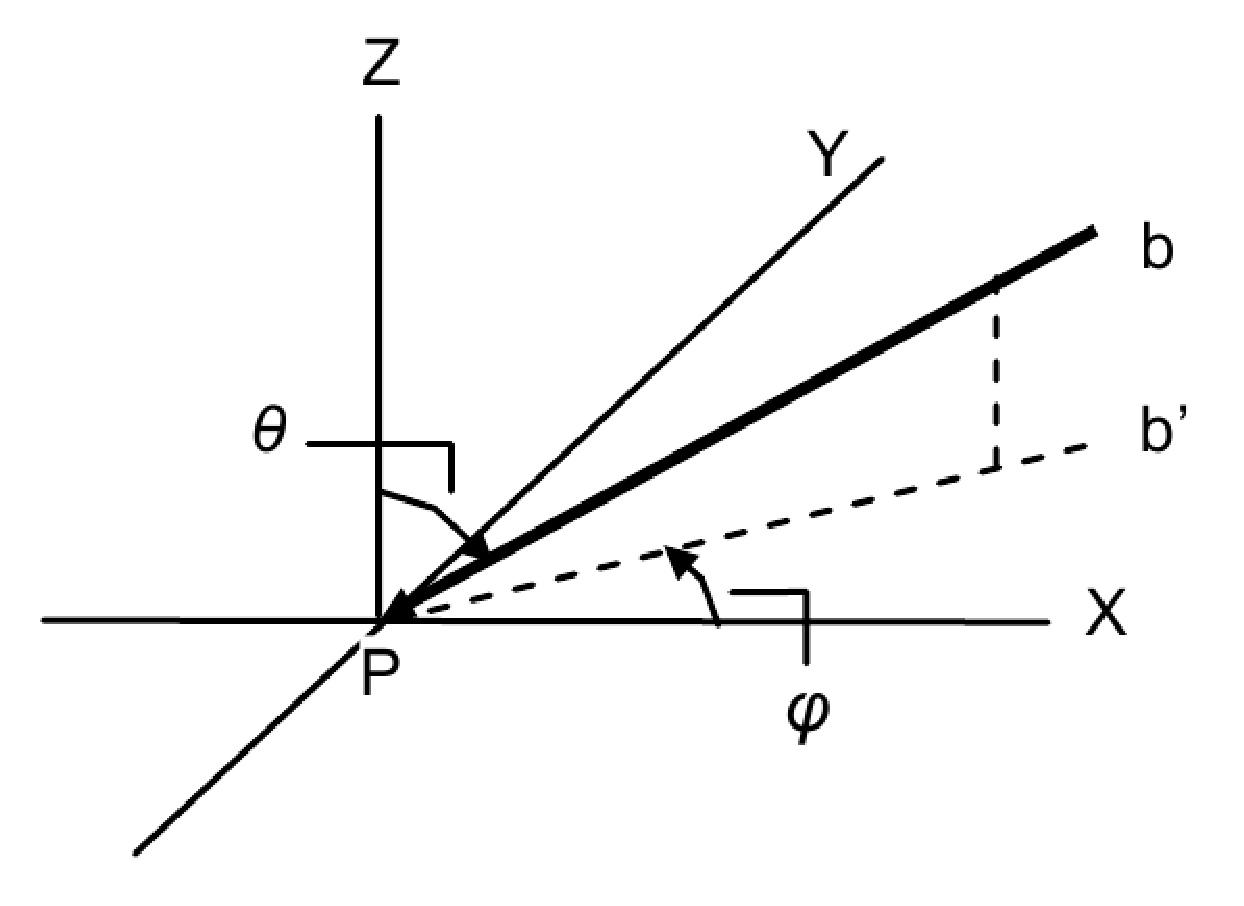
\includegraphics[scale=0.45]{shower_angles.eps}
\caption{The trajectory b of the primary particle and the shower can be described using the zenith angle $\theta$ (angle between Z-axis and b) and the azimuth angle $\varphi$ (angle between X-axis and b').}\label{fig:shower_angles}
\end{center}\end{figure}

\begin{shaded}
\textbf{Exercise \theExercise \stepcounter{Exercise}} : To determine the arrival times of the muons inside the air shower we need to make a few assumptions. The first is: the shower front is a flat surface. We shall call this surface S, which is perpendicular to the line b. The second assumption is: the surface of the Earth, from now on called A, is flat. Both surfaces are drawn in figure~\ref{fig:shower_surfaces.eps}. The third and last assumption is: the detectors are positioned at the same height.

Argue why these are reasonable assumptions (or simplifications). \\
\emph{Hint: What are the important properties of an air shower and the particles inside?}\end{shaded}

\section{First calculations}
Lets see how we can calculate both the zenith and azimuth angle from the arrival times measured at three detector stations.
\subsection{Zenith angle}
In figure~\ref{fig:shower_surfaces.eps} the shower front S moves with nearly the speed of light $c$ along the line b towards the surface of the Earth A. When the shower front reaches the surface it cuts though the surface along the line s. The arrival of the shower follows this line s.
As said before, the shower front moves with the speed of light, but the line s moves at a greater speed:
\begin{flalign}
v=\frac{c}{\sin \theta}
\label{eq:speed_s} 
\end{flalign}
because $\sin \theta \leq 1$: $v \geq c$ .

\begin{figure}\begin{center}
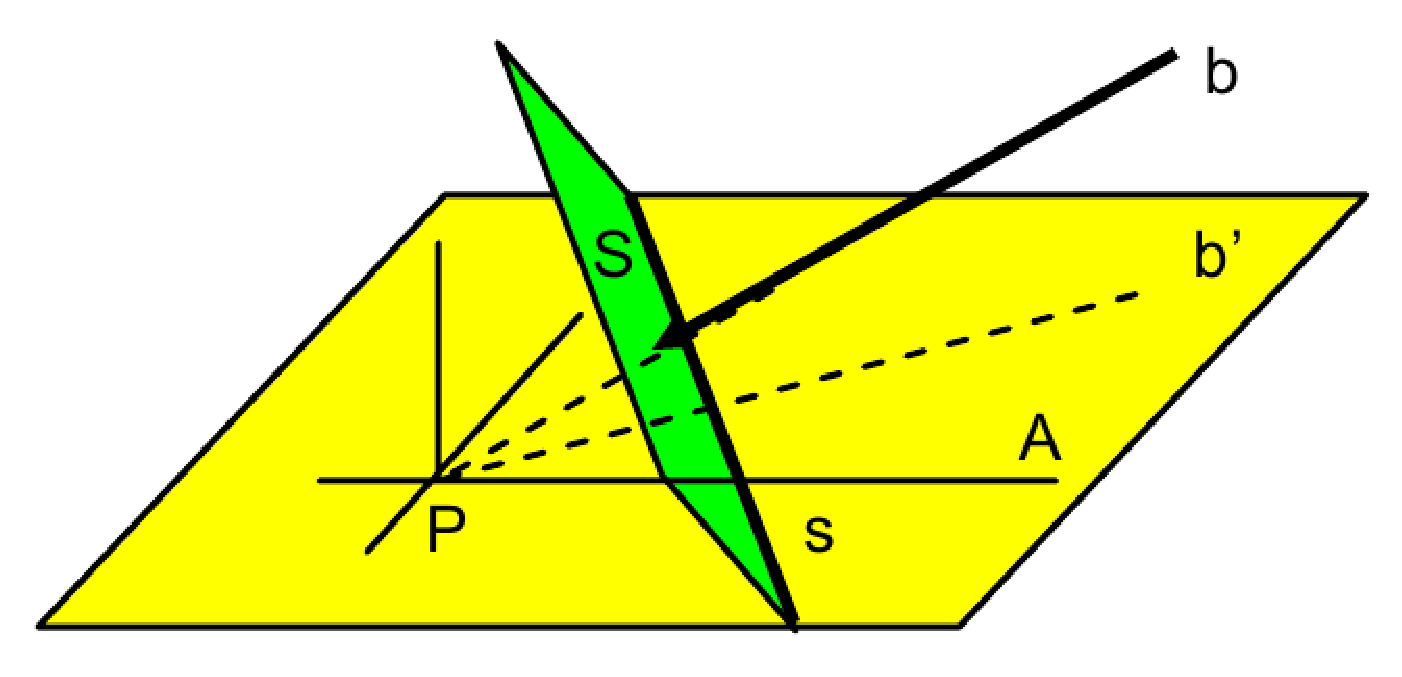
\includegraphics[scale=0.45]{shower_surfaces.eps}
\caption{The shower front S (green) is perpendicular to the shower trajectory b. It crosses the surface of the Earth A (yellow) along the line s. As the shower front travels along b the line s moves towards (and eventually past) the point P.}\label{fig:shower_surfaces.eps}
\end{center}\end{figure}

\begin{shaded}
\textbf{Exercise \theExercise \stepcounter{Exercise}} : The derivation of equation~\ref{eq:speed_s} is as follows: \\
Take a look at figure~\ref{fig:crosssection_BA.eps}, we have taken a cross section of figure~\ref{fig:shower_surfaces.eps} and placed it next to the original figure. The points P and Q both lie on the line b, but Q is placed `higher'. When the shower front S reaches point Q, it will be at point Q' on the surface. After a certain time $\Delta$t the shower front will reach P, the same is true for the line s. However the distance PQ' is larger than the distance PQ. \\
Use figure~\ref{fig:crosssection_BA.eps} to show that equation~\ref{eq:speed_s} is true. \end{shaded}

\begin{figure}[b]\begin{center}
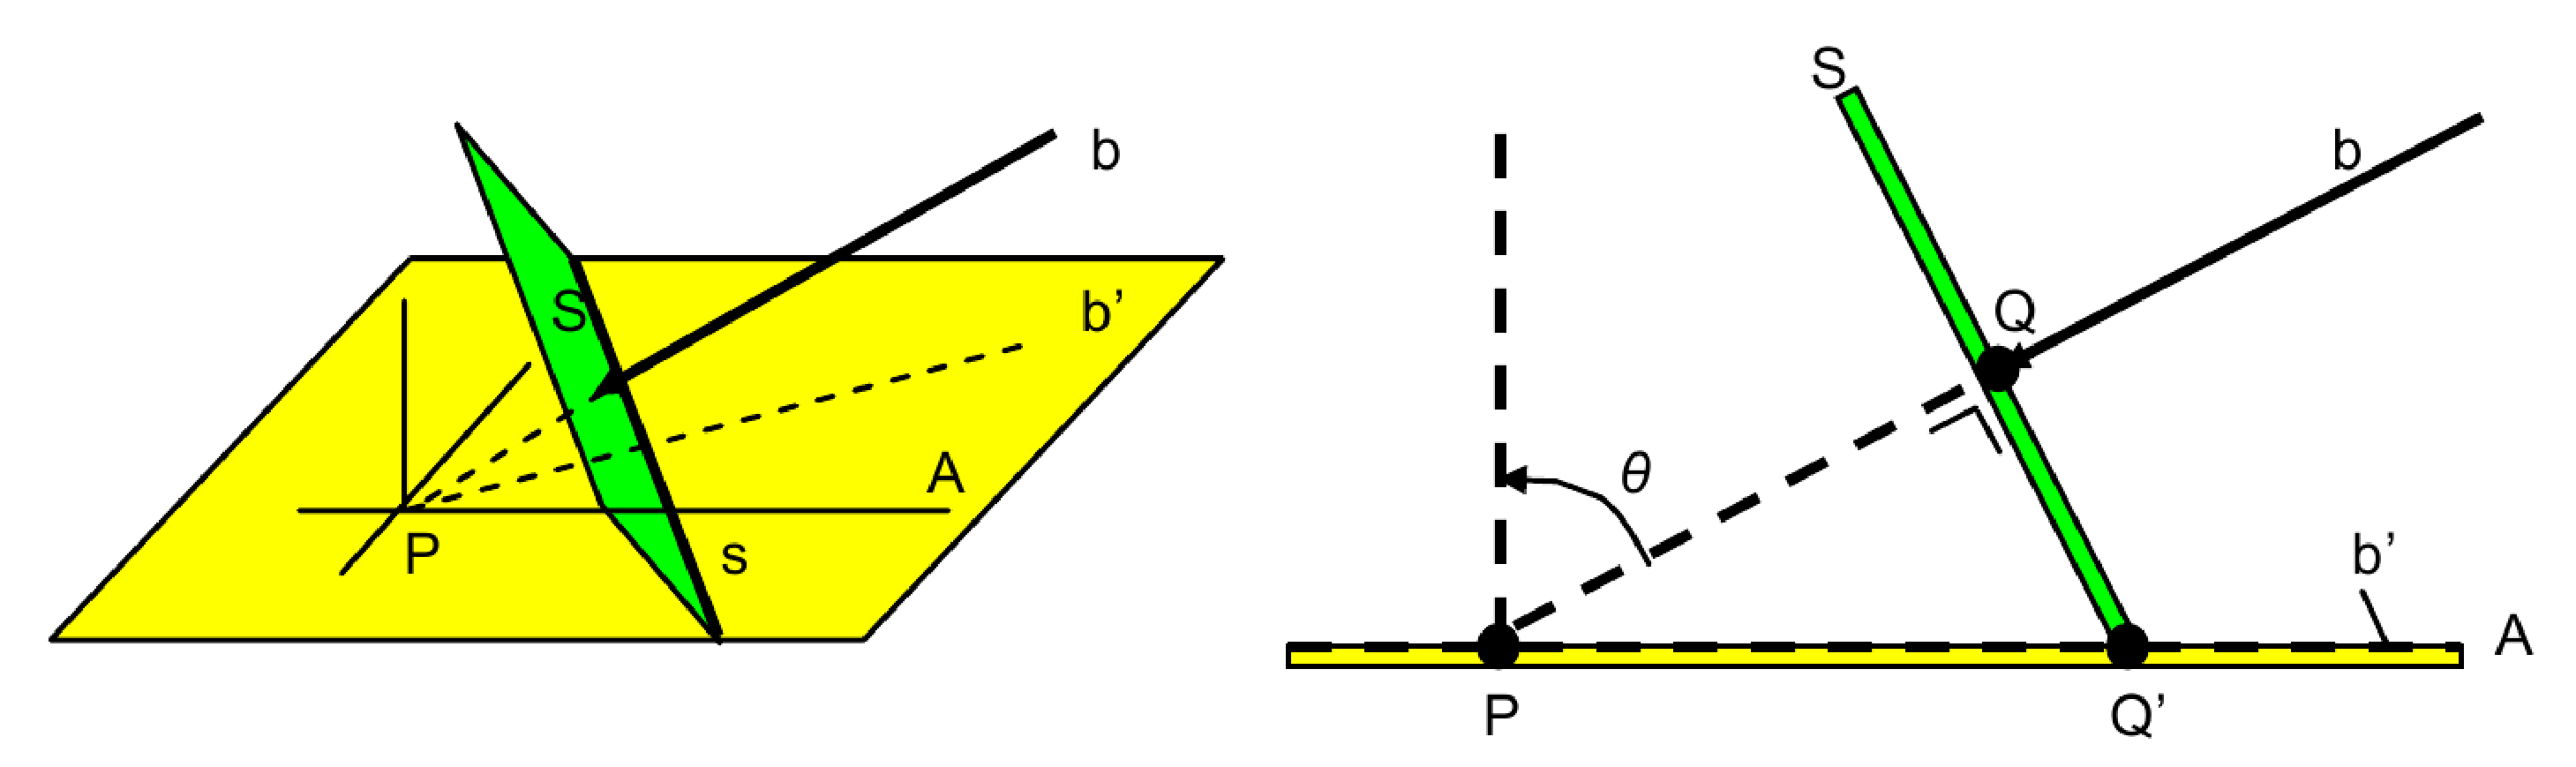
\includegraphics[scale=0.25]{crosssection_bA.eps}
\caption{The figure on the left is the same as figure~\ref{fig:shower_surfaces.eps}, the figure on the right is a cross section of this figure along the lines b and b'. The shower front S moves from Q towards P with the speed of light. After $\Delta$t time the front will reach P. In the same amount of time the line s moves from Q' to P.}\label{fig:crosssection_BA.eps}
\end{center}\end{figure}

The line s moves with a speed larger than $c$, this is an example of \textit{superluminal motion}. Although nothing can move faster than light (in vacuum) this specific type of faster than light travel is possible as we see daily with the HiSPARC network.

If we can determine the speed $v$ of the line s using the arrival times measured by our three detector stations, then the zenith angle can easily be calculated using equation~\ref{eq:speed_s}. However, before we can determine the speed of s, we first need to know the azimuth angle!

\subsection{Azimuth angle}
The line s between the shower front S and the surface of the Earth A has both a speed and direction. This direction is denoted by the angle $\xi$ between the line s and the X-axis. As shown in figure~\ref{fig:slope}. The angle $\xi$ is linked to the azimuth angle $\varphi$:
\begin{flalign}
\varphi = \xi - 90^{\circ} \label{eq:phi_xi}
\end{flalign}

\begin{figure}\begin{center}
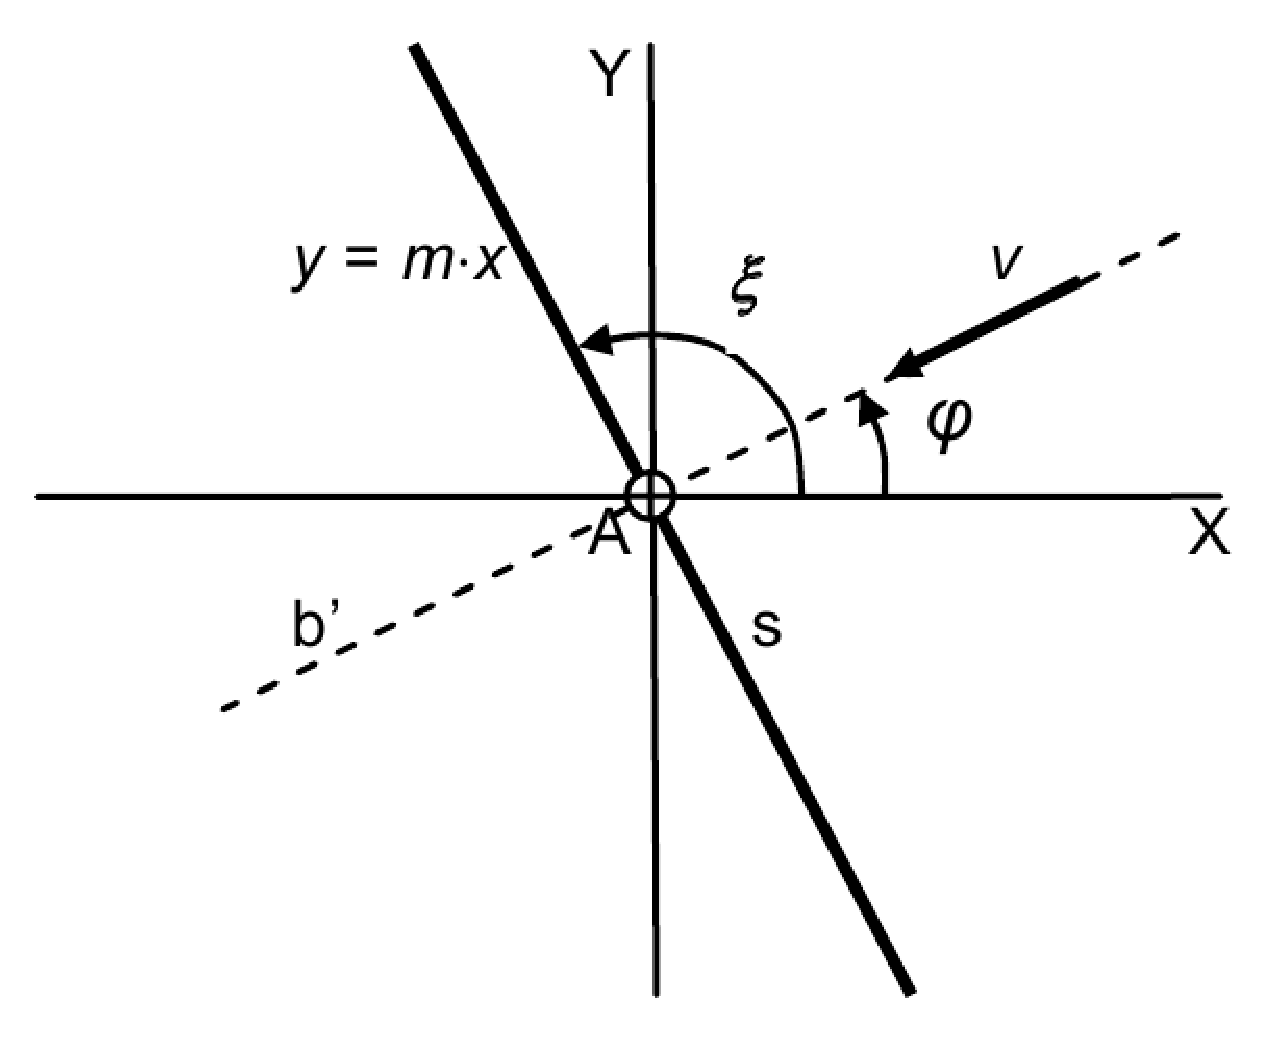
\includegraphics[scale=0.4]{slope.eps}
\caption{Calculating the azimuth angle. The equation for the line s through point A is given by $y = m \cdot x$. The slope $m$ is given by $m = \tan(\xi)$.}\label{fig:slope}
\end{center}\end{figure}

From figure~\ref{fig:slope} this should be clear: the azimuth angle is defined as the angle between the projection b' and the positive X-axis and the line s is perpendicular to this line.

If we can determine the angle $\xi$ using the data from three HiSPARC detector stations it is only a small step to calculate the azimuth angle $\varphi$ using equation~\ref{eq:phi_xi}.

\subsection{Detection}
We have three detector stations A, B, and C in the XY-plane, all have detected secondary particles created by the same shower. The recorded arrival times are $t_A$, $t_B$, and $t_C$. To make the following calculations a bit more organized we choose the arrival times such that $t_C > t_B > t_A$ and detector A is located at the centre of our coordinate system, both in space and time. This means that: $A(0,0,0)$. The data from stations B and C is as follows: $B(B_x,B_y,B_t)$ and $C(C_x,C_y,C_t)$ with $B_x=x_B-x_A$, $B_y=x_y-x_y$, $B_t=t_B-t_A$, $C_x=x_C-x_A$, $C_y=y_C-y_A$, and $C_t=t_C-t_A$.

The line s crosses the origin of the coordinate system at $t=0$. The equation describing this line is as follows: $y=m \cdot x$, with $m$ the slope of the line: $m=\tan \xi$ (see figure~ \ref{fig:slope}).

There is a standard procedure to determine the distance between an arbitrary point and the line s in the XY-plane. Applying this procedure to the points B en C (see figure~\ref{fig:distances}) yields the following results:
\begin{flalign}
d_B = \frac{B_y - m \cdot B_x}{\sqrt{m^ 2 +1}} \label{eq:d_B}\\
d_C = \frac{C_y - m \cdot C_x}{\sqrt{m^ 2 +1}} \label{eq:d_C}
\end{flalign}

But we have a little more informations about these distances. We know that the line s travels at a certain speed, which means that we can calculate the time it take s to travel these distances: $d_B = v \cdot B_t$ and $d_C = v \cdot C_t$. Combining this with equations~\ref{eq:d_B} and \ref{eq:d_C} yields the following result:
\begin{flalign}
\frac{B_y - m \cdot B_x}{\sqrt{m^2 +1}} = v \cdot B_t \label{eq:d_B_t} \\
\frac{C_y - m \cdot C_x}{\sqrt{m^2 +1}} = v \cdot C_t\label{eq:d_C_t}
\end{flalign}

In equations~\ref{eq:d_B_t} and \ref{eq:d_C_t} we have two unknowns: $m$ and $v$. We can rearrange the two equations to solve for the two unknowns:
\begin{flalign}
m &= \frac{C_y \cdot B_t - B_y \cdot C_t}{C_x \cdot B_t - B_x \cdot C_t} \label{eq:m} \\
v &= \frac{C_y - m \cdot C_x}{C_t \cdot \sqrt{m^2 +1}} \label{eq:v}
\end{flalign}

Equation~\ref{eq:m} allows us to calculate the slope $m$ of the line between the shower front S and the Earth surface A using the space and time coordinates of detector station B and C (with respect to A). From this follows the angle $\xi$: $m=\tan \xi$, which can be rearranged to $\xi=\arctan m$. We can then use equation~\ref{eq:phi_xi} to calculate the azimuth angle of the primary cosmic ray:
\begin{flalign}
\varphi = \arctan \left( m - 90^{\circ} \right) \label{eq:varphi}
\end{flalign}

\begin{figure}\begin{center}
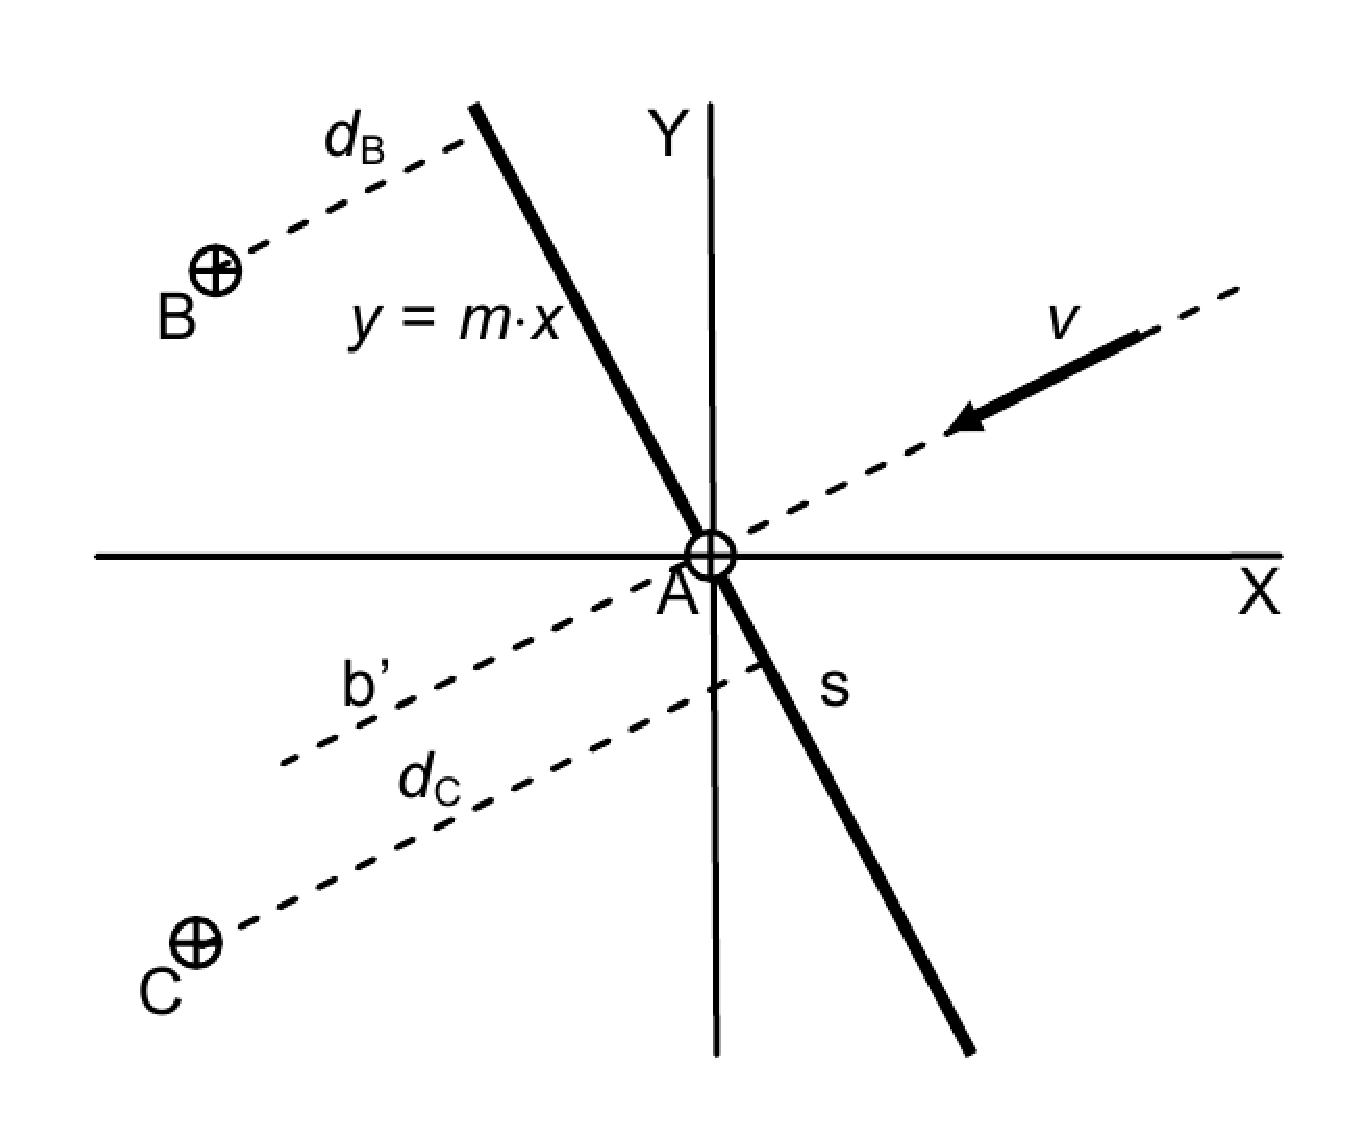
\includegraphics[scale=0.4]{distances.eps}
\caption{We can use a standard method to determine the distances $d_B$ and $d_C$ between the line s and the points B and C respectively.}\label{fig:distances}
\end{center}\end{figure}

Once the slope $m$ is known we can solve equation~\ref{eq:v} giving us the speed at which the line s travels across the Earth surface. This allows us to solve equation~\ref{eq:speed_s} for the angle $\theta$:
\begin{flalign}
\theta = \arcsin \left( \frac{c}{v} \right) \label{eq:theta}
\end{flalign}
By solving equations~\ref{eq:m}, \ref{eq:v}, \ref{eq:varphi}, and \ref{eq:theta} using the location and time coordinates of the (three) detector stations we have determined the direction of the primary cosmic particle.

\begin{shaded}
\textbf{Exercise \theExercise \stepcounter{Exercise}} : Equations~\ref{eq:d_B} and \ref{eq:d_C} give us the distances $d_B$ and $d_C$ between the line s and the points B and C. The equations were derived using a standard procedure which allows one to calculate the distance between an arbitrary point in the XY-plane and a line through the origin A.

Give the derivation of these equations.\\
\emph{A few hints:
\begin{enumerate}[-]
\item Start with the equation for the line s ($y=m \cdot x$).
\item Give the equation for the line through B and perpendicular to s.
\item Give a similar equation for the line though C.
\item Calculate the coordinates where these two lines intersect s.
\item Use these coordinates to calculate the distances $d_B$ or $d_C$. \end{enumerate}}
\end{shaded}

\begin{shaded}
\textbf{Exercise \theExercise \stepcounter{Exercise}} : Equations~\ref{eq:m} and \ref{eq:v} give the solutions of the system of equations~\ref{eq:d_B_t} and \ref{eq:d_C_t}.

Verify that this solutions is correct. \end{shaded}

\begin{shaded}
\textbf{Exercise \theExercise \stepcounter{Exercise}} : The directions of the primary cosmic particle (consisting of the two angles $\varphi$ and $\theta$) can be determined using equations~\ref{eq:m} through \ref{eq:theta}. In table~\ref{tab:data_1} the data of a simulated coincidence measurement is shown. The place coordinates ($x$ and $y$) are given with respect to an arbitrary point. In a similar fashion, the arrival time ($t$) is measured from an arbitrary point of time.

Calculate the direction of the primary particle for the data in the given table.\\
\emph{A few tips if you do not know how to tackle this problem:
\begin{enumerate}[-]
\item Decide which station is A, which is B, and which is C. Adjust the coordinate system accordingly.
\item Sketch the layout of the detector stations. Draw an estimation of the line s through the origin. This will help you in determining the correct values of $\xi$ and $\varphi$ when solving equations~\ref{eq:m} and \ref{eq:varphi}. The results of your calculations might be a negative angle: an angle between the positive X-axis and the line s in a clockwise fashion. When you look at figure~\ref{fig:slope} you see that the angles should turn in a anticlockwise fashion. Your end result should conform to the drawing in figure~\ref{fig:slope}.
\item Equation~\ref{eq:v} might yield a negative result for the speed $v$ of the shower front across the Earth surface. This indicates the direction of travel of the front. However, for the calculation of the angel $\theta$ with equation~\ref{eq:theta} this direction is not important, this information is contained in the angle $\varphi$. Therefore, use the absolute value of $v$ in your calculation.
\end{enumerate}}
\end{shaded}

\begin{tabular}[h] {l r r r}
Detector station & $x$-coordinate~(m) & $y$-coordinate~(m) & arrival time $t$~(\textmu s) \\ \hline
1 & 400 & 150 & 11.01\\
2 & 500 & -400 & 11.14\\
3 & 800 & 100 & 10.72\\
\end{tabular}
\captionof{table}{HiSPARC sample data for exercise 5.}\label{tab:data_1}

\begin{shaded}
\textbf{Exercise \theExercise \stepcounter{Exercise}} : In the night of 18 July 2004 the HiSPARC-cluster Nijmegen registered the first threefold coincidence.\footnotemark In the table below the data from this event are shown. For convenience detector station A is already placed at the origin of the coordinate system. Use this data to determine the direction of the primary cosmic ray.\end{shaded}

\footnotetext{Three different detector stations measured particles from the same air shower.}

\begin{tabular}[h] {l r r r}
Detector station & $x$-coordinate~(m) & $y$-coordinate~(m) & arrival time $t$~(\textmu s) \\ \hline
A & 0.0 & 0.0 & 52.7\\
B & 438.8 & 277.6 & 52.8\\
C & 282.1 & -749.4 & 53.9\\
\end{tabular}
\captionof{table}{First HiSPARC threefold coincidence event data for exercise 6.}\label{tab:data_2}

\end{document}